\section{Introduzione}

\subsection{Descrizione generale del sito}

Il sistema oggetto di analisi è la piattaforma web \textit{BrainBox}, sviluppata con lo scopo di fornire agli studenti universitari un ambiente digitale integrato per supportare e ottimizzare le loro attività di studio. Il contenuto funzionale e informativo del sistema è composto da:

\begin{itemize}
    \item Un archivio di materiale didattico dove gli utenti possono caricare e gestire i propri appunti personali, con la possibilità di renderli pubblici per la consultazione da parte della \textit{community}.
    
    \item Una sezione dedicata alla trascrizione automatica di lezioni registrate, che utilizza servizi di intelligenza artificiale per convertire file audio in formato testuale.
    
    \item Uno strumento per la sintesi vocale, che permette di trasformare qualsiasi contenuto testuale, come appunti o trascrizioni, in un file audio ascoltabile.
    
    \item Un'area di pianificazione personale dove gli utenti possono creare e monitorare piani di studio in vista degli esami.
    
    \item Un sistema di interazione sociale che permette di aggiungere commenti ai documenti condivisi, facilitando il feedback e la discussione.
\end{itemize}

Per organizzare al meglio queste funzionalità, il sito è stato diviso in queste sezioni principali:

\begin{itemize}
    \item \textbf{Homepage}: la pagina iniziale da cui si effettua il login o la registrazione. Sezione \ref{homepage}.
    
    \item \textbf{Registrazione e Login}: le due pagine che permettono all'utente di registrare i propri dati e creare un proprio profilo \textit{BrainBox} oppure autenticarsi. Sezione \ref{login_registrazione}.
    
    \item \textbf{Dashboard}: la pagina principale visibile dopo l'accesso, che fa da punto di partenza per navigare in tutto il sito. Sezione \ref{dashboard}.
    
    \item \textbf{I Miei Appunti}:  l'archivio personale in cui l'utente può vedere e gestire i file che ha caricato. Sezione \ref{miei_appunti}.
    
    \item \textbf{Dettaglio Documento}: la pagina per leggere un singolo appunto, scaricarne il file e lasciare commenti. Sezione \ref{dettaglio_documento}.
    
    \item \textbf{Esplora Appunti}: la sezione per cercare e consultare i documenti resi pubblici dagli altri utenti. Sezione \ref{subsubsec:esplora_appunti}.
    
    \item \textbf{Sbobinatore AI}: la pagina in cui caricare un file audio per ottenerne la trascrizione in automatico. Sezione \ref{strumentiAI}.
    
    \item \textbf{Generatore AudioNote}: l'area dove inserire un testo per trasformarlo in un file audio. Sezione \ref{strumentiAI}.
    
    \item \textbf{StudyFlow}: la sezione per creare e pinificare i propri esami includendo il piano di studio (task e materiale di studio) e tenere d'occhio le scadenze. Sezione \ref{study_flow}.
    
    \item \textbf{Profilo Utente}: la sezione in cui l'utente può gestire il proprio profilo \textit{BrainBox} visualizzando o modificando i propri dati personali. Sezione \ref{profilo_utente}.
\end{itemize}

Le principali funzionalità sono accessibili solo all'utente registrato previa autenticazione. Queste pagine verranno descritte nel dettaglio nei capitoli successivi.

Per l'utente registrato sarà possibile interagire con tutte le funzionalità del sistema: più precisamente, questo tipo di utente può creare, visualizzare, modificare ed eliminare i propri appunti; visualizzare e ricercare gli appunti pubblici degli altri utenti; creare, modificare ed eliminare i propri commenti; e utilizzare gli strumenti AI di trascrizione.

Per l'utente visitatore (non autenticato), sarà possibile esclusivamente visualizzare la Homepage del sito e da lì accedere alle pagine per effettuare il Login o la Registrazione.

\subsection{Descrizione delle sezioni principali}

L'architettura informativa del sistema \textit{BrainBox} è organizzata attorno a un'area ad accesso riservato, che racchiude tutte le funzionalità principali. La navigazione all'interno di quest'area è gestita da una barra di navigazione persistente che garantisce un accesso coerente e prevedibile alle diverse sezioni.

\subsubsection{Homepage}
\label{homepage}
La Homepage funge da portale d'ingresso pubblico al sistema (Figura \ref{fig:1-1}). La sua interfaccia è minimale e ha lo scopo di indirizzare l'utente verso il processo di autenticazione. I suoi componenti principali sono i due link distinti per la Registrazione di un nuovo account e il Login per gli utenti già registrati. Presenta altri contenuti informativi come \textit{pricing} e funzionalità.

    \begin{figure}[H]
        \centering
        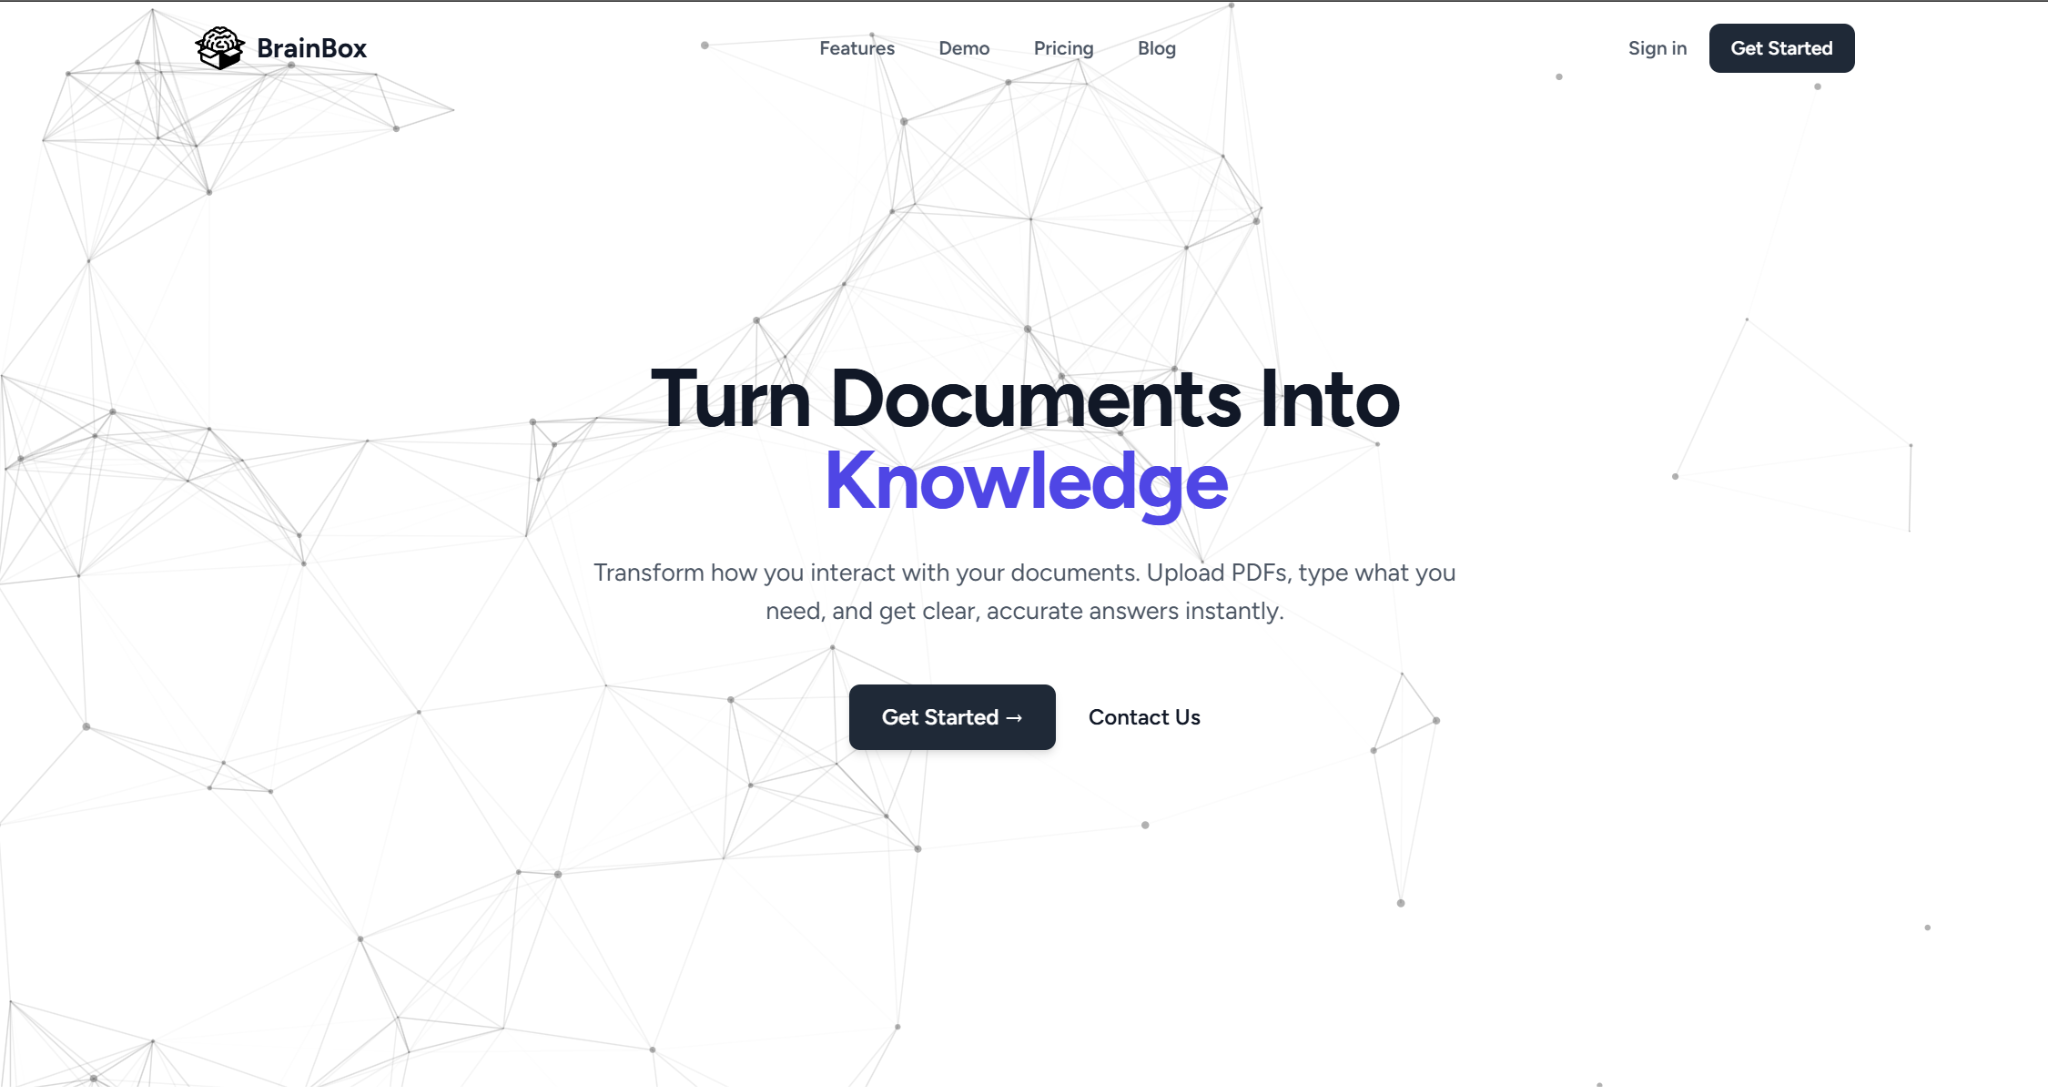
\includegraphics[width=0.8\textwidth]{figures/01-introduzione/immagine_1.png}
        \caption{Homepage.}
        \label{fig:1-1}
    \end{figure}

I componenti più importanti di questa sezione sono:

\begin{itemize}
    \item \textbf{Barra di navigazione (Figura \ref{fig:1-2})}: all'interno di questa barra collocata nella parte superiore di tutte le pagine si trovano tutte le sezioni fra le quali un qualsiasi visitatore può navigare;
    
    \begin{figure}[H]
        \centering
        
\includegraphics[width=0.8\textwidth]{figures/01-introduzione/immagine_2.png}
        \caption{Barra di navigazione.}
        \label{fig:1-2}
    \end{figure}
    
    \item \textbf{Footer (Figura \ref{fig:1-3}):} è una sezione collocata nella parte finale delle pagine del sito che racchiude i \textit{link} di navigazione, i contatti e i riferimenti social dell'associazione.

    \begin{figure}[H]
        \centering
        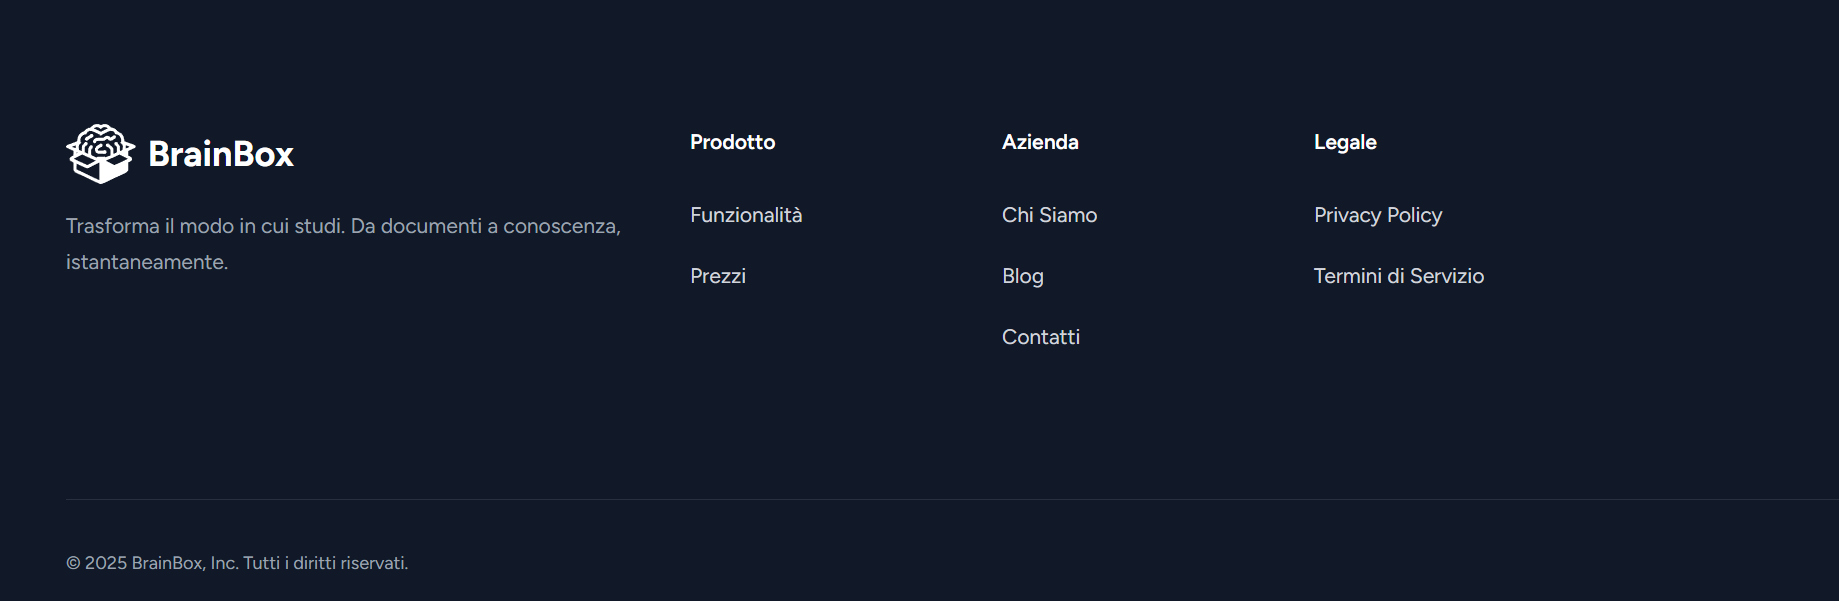
\includegraphics[width=0.8\textwidth]{figures/01-introduzione/immagine_3.png}
        \caption{Footer.}
        \label{fig:1-3}
    \end{figure}
    
    \item \textbf{Pricing (Figura \ref{fig:1-4}):} è una sezione dedicata agli abbonamenti, che mostra come sono divisi i servi tra i vari piani.

    \begin{figure}[H]
        \centering
        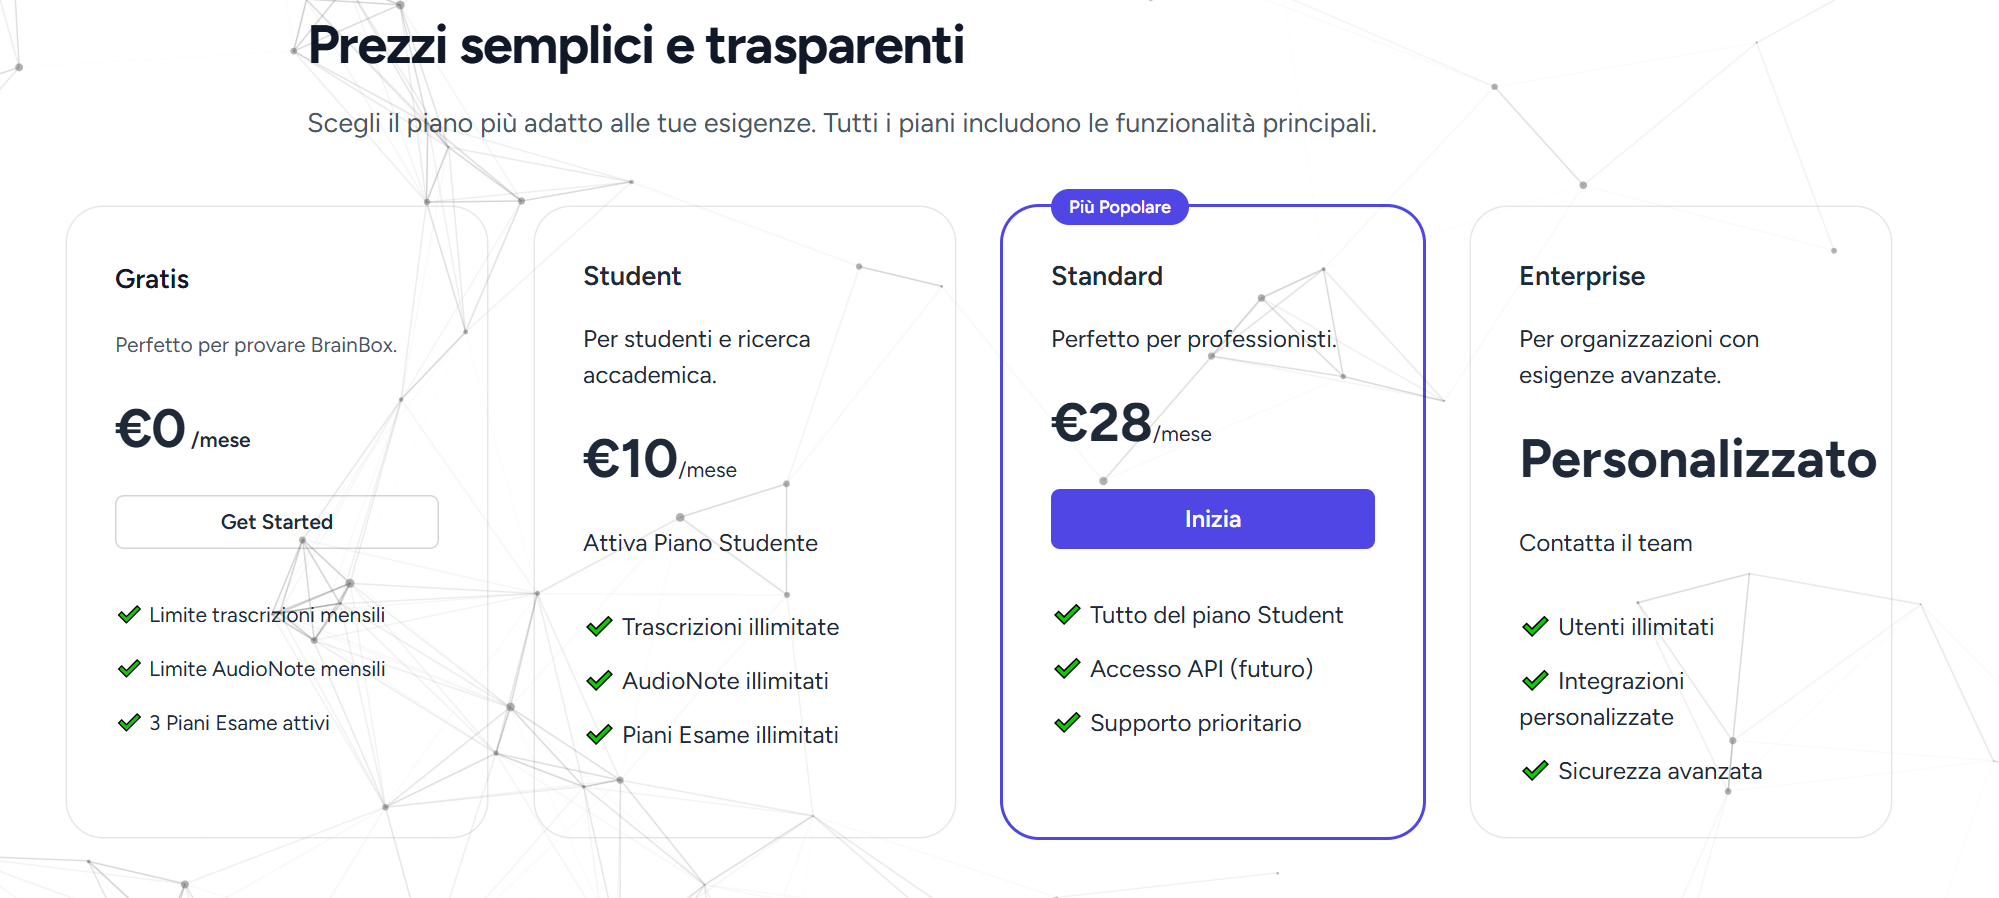
\includegraphics[width=0.8\textwidth]{figures/01-introduzione/immagine_4.png}
        \caption{Pricing.}
        \label{fig:1-4}
    \end{figure}
    
    \item \textbf{Funzionalità (Figura \ref{fig:1-5}):} è una sezione che mostra panoramica delle principali funzionalità offerte dalla piattaforma, che includono la gestione documentale e gli strumenti di automazione basati su IA.

    \begin{figure}[H]
        \centering
        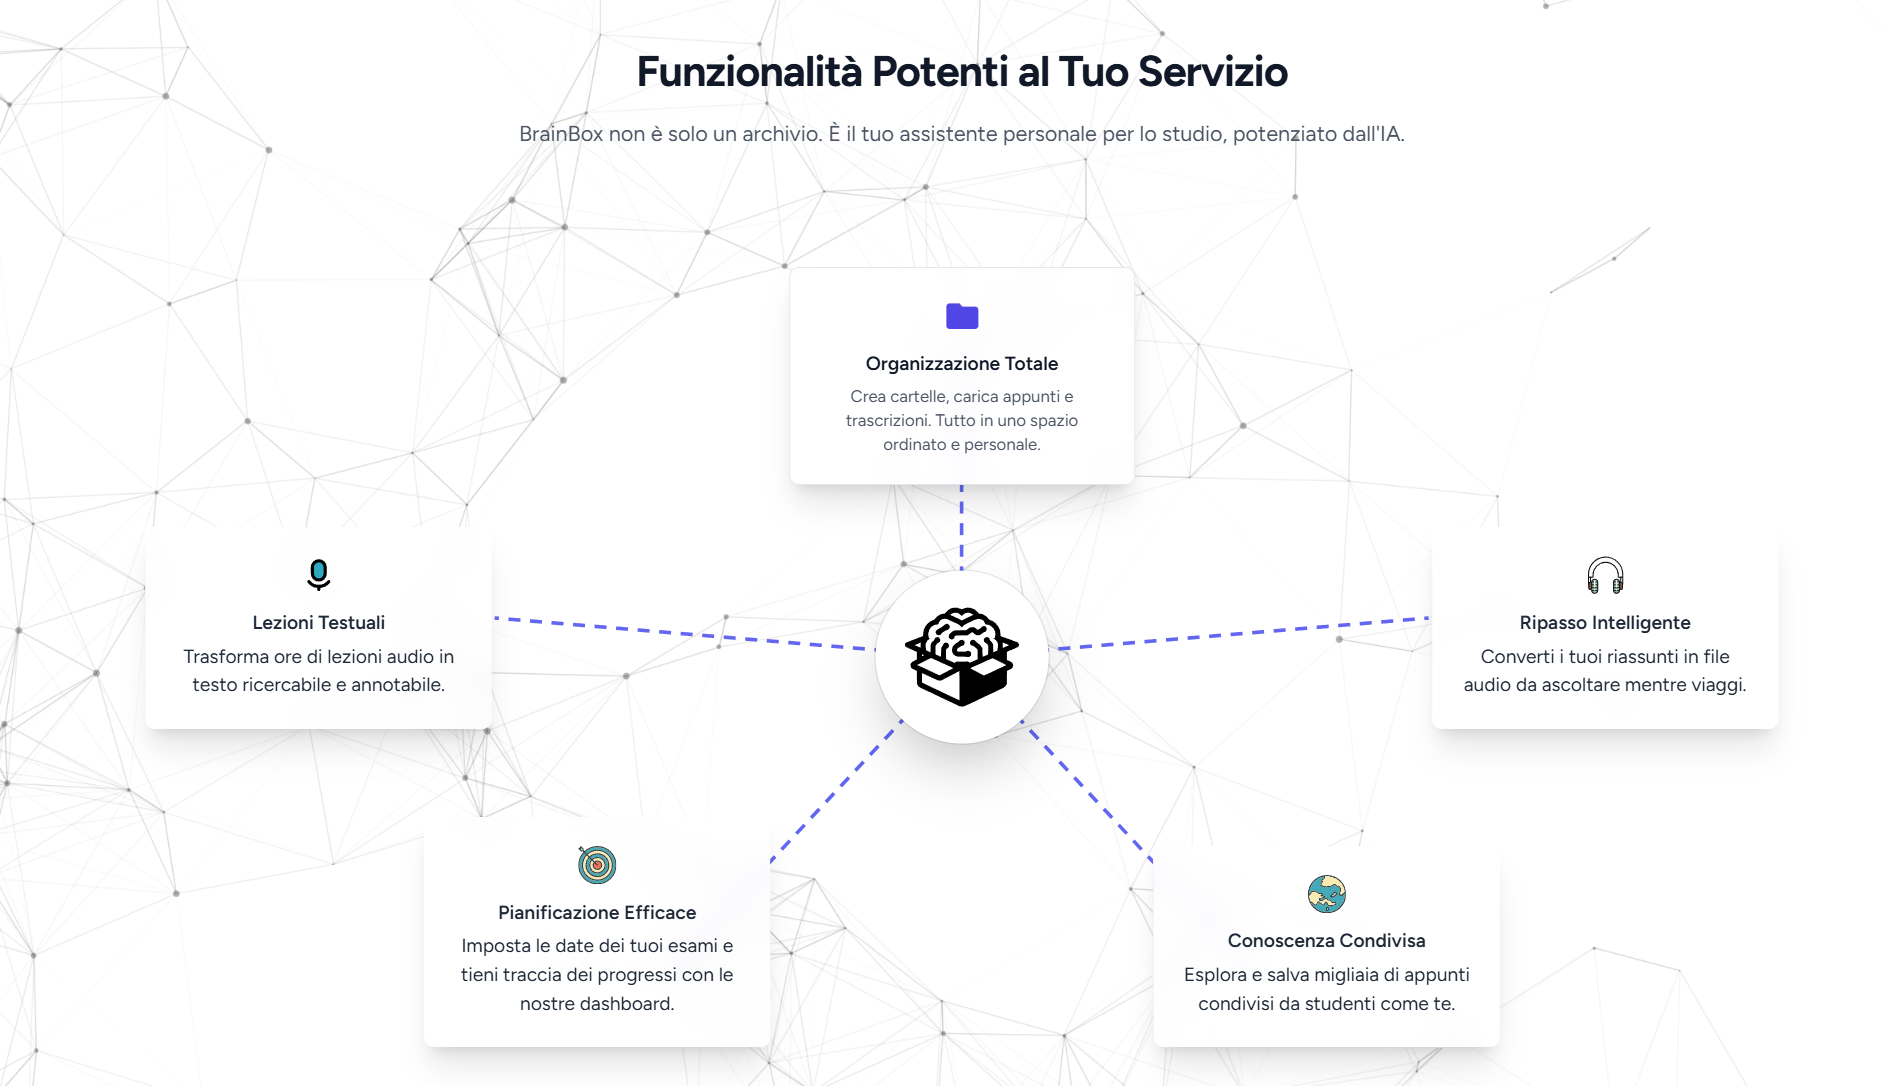
\includegraphics[width=0.8\textwidth]{figures/01-introduzione/immagine_5.png}
        \caption{Funzionalità.}
        \label{fig:1-5}
    \end{figure}
    
    \item \textbf{Call to action (Figura \ref{fig:1-6}):} è un'interfaccia posizionata strategicamente per incoraggiare la registrazione o l'accesso alla piattaforma.

    \begin{figure}[H]
        \centering
        
\includegraphics[width=0.8\textwidth]{figures/01-introduzione/immagine_6.png}
        \caption{Call to action.}
        \label{fig:1-6}
    \end{figure}
\end{itemize}

\subsubsection{Pagine di Login e Registrazione}
\label{login_registrazione}
Queste due interfacce sono composte da form standard per la gestione dell'identità dell'utente. La \textbf{pagina di Login} richiede l'inserimento di  \textit{email} e \textit{password} per consentire l'accesso agli utenti già registrati. La \textbf{pagina di Registrazione} è un processo a due fasi: la prima richiede le credenziali base per la creazione del profilo (nome, indirizzo \textit{email}, \textit{password}), mentre la seconda fase è dedicata alla raccolta di \textit{metadati} specifici del contesto accademico, quali Università di provenienza, Dipartimento e Ciclo di studi. Entrambe le interfacce gestiscono la validazione dei dati e forniscono un \textit{feedback} testuale immediato in caso di errori di inserimento (es. credenziali errate, formato email non valido).

    \begin{figure}[H]
        \centering
        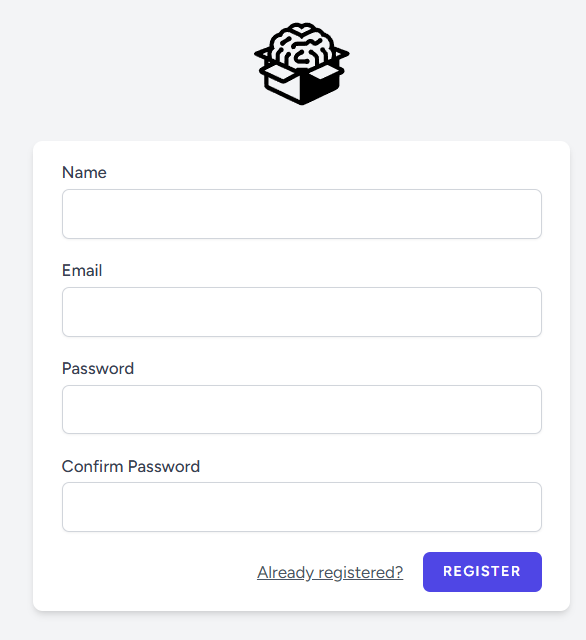
\includegraphics[width=0.8\textwidth]{figures/01-introduzione/immagine_7.png}
        \caption{Prima fase del processo di Registrazione, focalizzata sulla creazione dell'account utente tramite l'inserimento delle credenziali di base.}
        \label{fig:1-7}
    \end{figure}

    \begin{figure}[H]
        \centering
        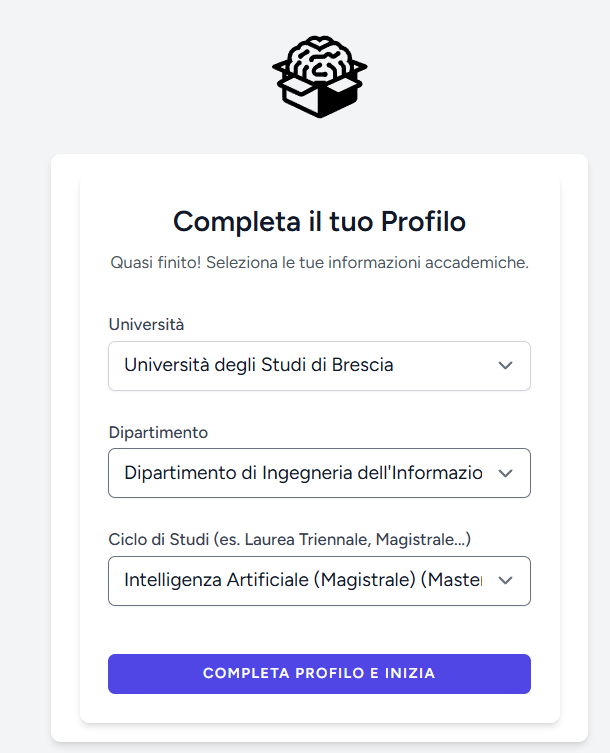
\includegraphics[width=0.8\textwidth]{figures/01-introduzione/immagine_8.png}
        \caption{Seconda fase del processo di Registrazione, dedicata alla profilazione dell'utente attraverso la raccolta di \textit{metadati} accademici.}
        \label{fig:1-8}
    \end{figure}

    \begin{figure}[H]
        \centering
        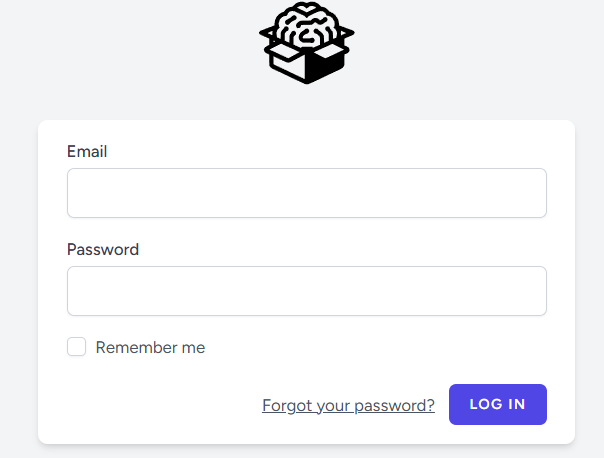
\includegraphics[width=0.8\textwidth]{figures/01-introduzione/immagine_9.png}
        \caption{Interfaccia del form di Login, che richiede le credenziali standard (\textit{email} e \textit{password}) per l'autenticazione dell'utente.}
        \label{fig:1-9}
    \end{figure}

\subsubsection{Dashboard}
\label{dashboard}
La Dashboard è la prima pagina che l'utente visualizza dopo aver completato con successo l'autenticazione e agisce come \textit{hub} centrale dal quale si diramano tutte le navigazioni successive. La sua struttura è organizzata su due componenti principali:

\begin{itemize}
    \item Una barra di navigazione verticale (\textit{sidebar}) persistente, che contiene i \textit{link} diretti a tutte le macro-funzionalità del sito (\textit{I Miei Appunti}, \textit{Esplora Appunti}, \textit{StudyFlow} e \textit{strumenti AI}), garantendo un accesso costante da qualsiasi punto dell'applicazione.
    
    \begin{figure}[H]
        \centering
        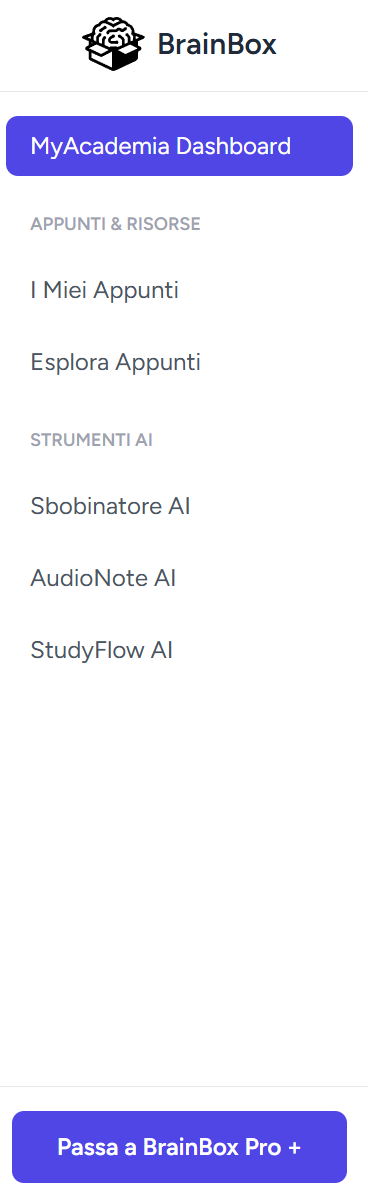
\includegraphics[width=0.3\textwidth]{figures/01-introduzione/immagine_10.png}
        \caption{Barra di navigazione verticale (\textit{sidebar})}
        \label{fig:1-10}
    \end{figure}
    
    \item Un'area centrale che fa da vero e proprio pannello di controllo per l'utente. Qui si trova un riassunto delle informazioni più utili tramite dei \textit{widget} (come gli ultimi appunti caricati o le prossime scadenze), insieme a una serie di scorciatoie per accedere rapidamente alle funzioni principali della piattaforma.
    
    \begin{figure}[H]
        \centering
        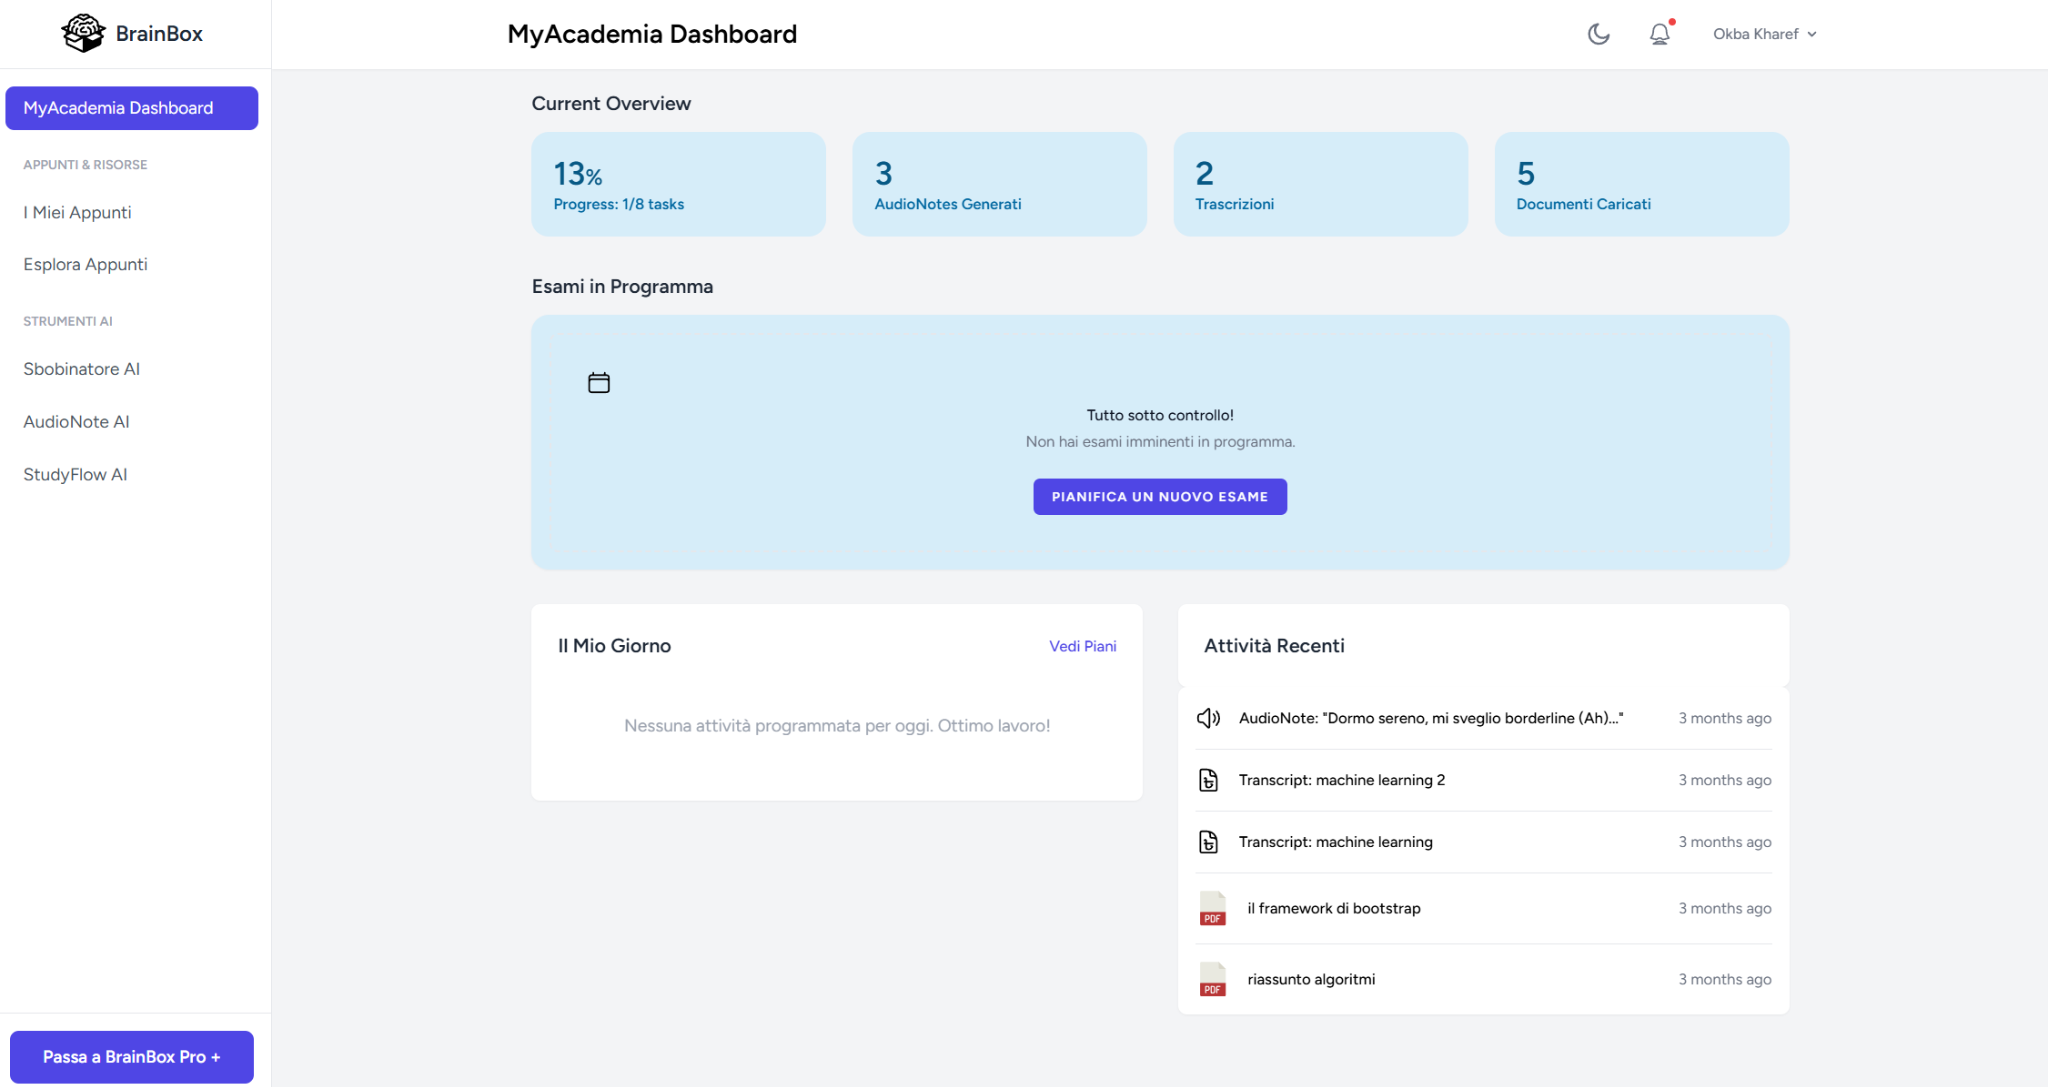
\includegraphics[width=0.8\textwidth]{figures/01-introduzione/immagine_11.png}
        \caption{Panoramica della \textit{Dashboard}, che mostra la struttura a due colonne con la navigazione laterale e l'area centrale contenente \textit{widgets} di riepilogo e scorciatoie.}
        \label{fig:1-11}
    \end{figure}
\end{itemize}

\subsubsection{Sezione Esplora Appunti}
\label{subsubsec:esplora_appunti}
Questa sezione rappresenta il cuore collaborativo della piattaforma. Il suo scopo è permettere la scoperta e la consultazione dei documenti condivisi dalla \textit{community}. L'elemento principale della pagina è una grande barra di ricerca, che permette di filtrare gli appunti per titolo o materia. Subito sotto si trova la lista dei documenti pubblici, mostrati sotto forma di \textit{card} con le informazioni essenziali (titolo, materia, autore) e il collegamento per aprire il singolo dettaglio.

    \begin{figure}[H]
        \centering
        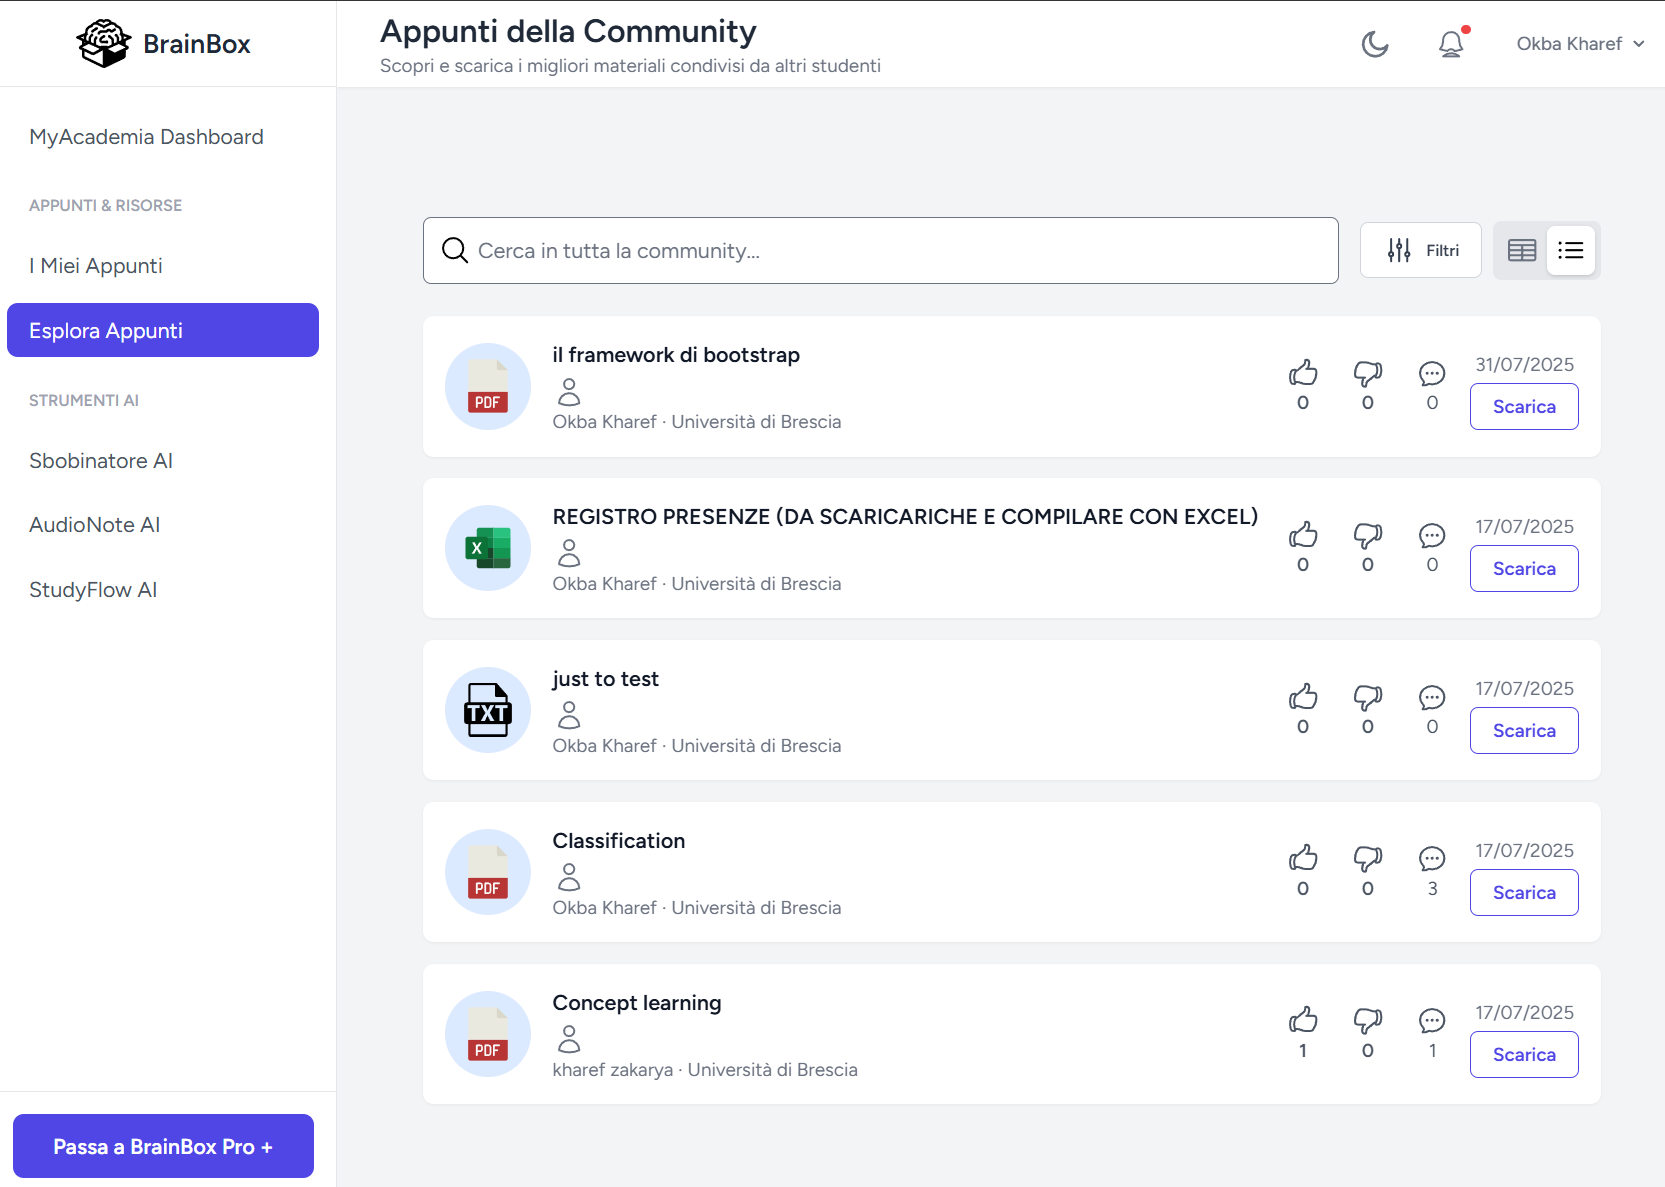
\includegraphics[width=0.8\textwidth]{figures/01-introduzione/immagine_12.png}
        \caption{Interfaccia della pagina \textit{Esplora Appunti}, che mostra il campo di ricerca testuale per il filtraggio e la presentazione dei documenti pubblici attraverso una griglia di \textit{card} informative.}
        \label{fig:1-12}
    \end{figure}

\subsubsection{Sezione I Miei Appunti}
\label{miei_appunti}
Questa pagina costituisce l'archivio personale dell'utente. La sua struttura è simile a quella della pagina \textit{Esplora Appunti} (Sezione \ref{subsubsec:esplora_appunti}), ma l'elenco è filtrato per mostrare esclusivamente i documenti caricati dall'utente autenticato. Per ogni documento elencato, sono presenti controlli specifici per la gestione, ovvero i pulsanti di \textit{modifica} ed \textit{elimina}. Un pulsante di azione primario (\textit{CARICA FILE}) permette all'utente di accedere al form di caricamento di un nuovo documento.

    \begin{figure}[H]
        \centering
        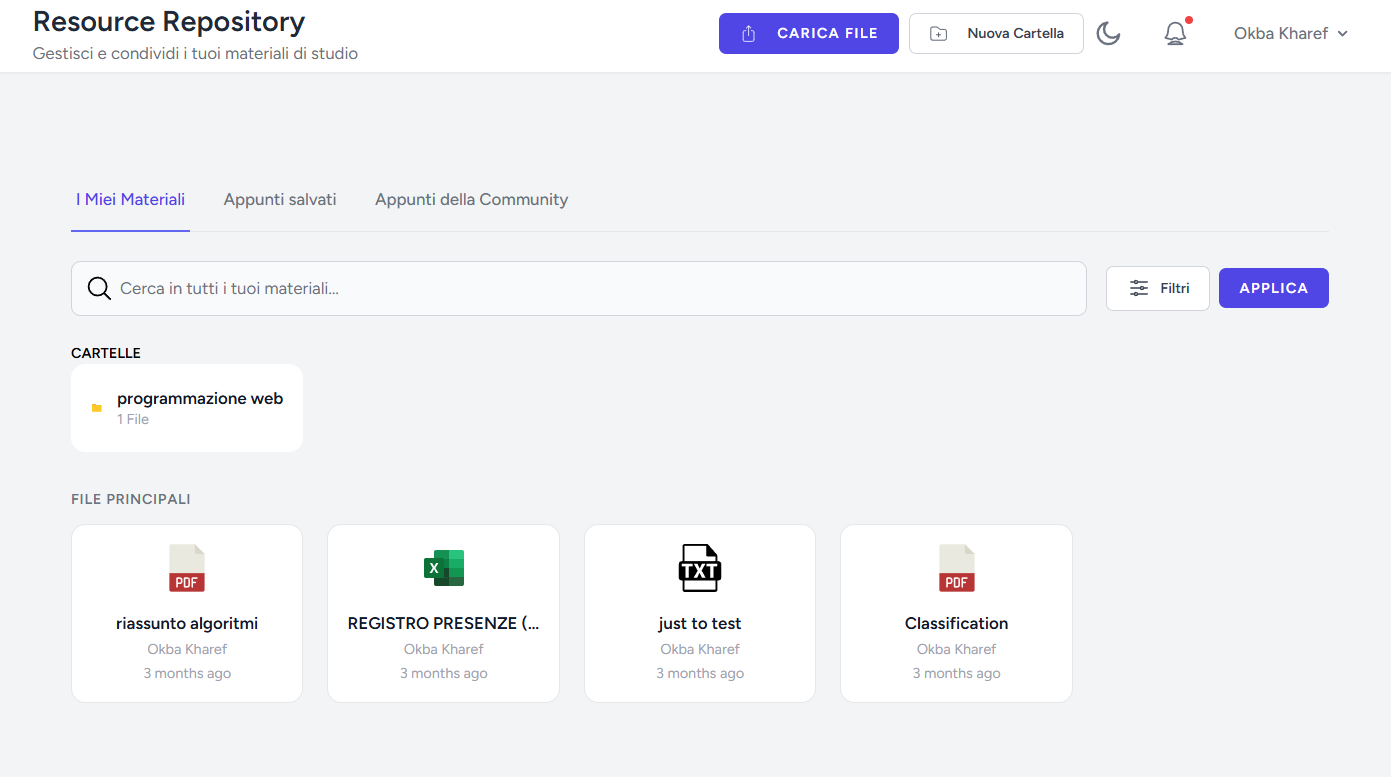
\includegraphics[width=0.8\textwidth]{figures/01-introduzione/immagine_13.png}
        \caption{Interfaccia della pagina \textit{I Miei Appunti}, l'archivio personale dove l'utente visualizza e gestisce i propri documenti.}
        \label{fig:1-13}
    \end{figure}

\subsubsection{Pagina di Dettaglio del Documento}
\label{dettaglio_documento}
Questa interfaccia è dedicata alla consultazione approfondita di un singolo documento. È suddivisa in tre aree funzionali distinte:

\begin{itemize}
    \item Un'area informativa superiore che riassume i \textit{metadati} dell'appunto: titolo, materia, autore, descrizione e un link per il download del file.
    
    \item Un'area di interazione contenente il form per l'inserimento di nuovi commenti.
    
    \item Un'area di consultazione inferiore che elenca tutti i commenti esistenti in ordine cronologico, con l'indicazione dell'autore e della data. Per i commenti di proprietà dell'utente, sono presenti i controlli per la modifica e l'eliminazione \textit{in-place}.
\end{itemize}

    \begin{figure}[H]
        \centering
        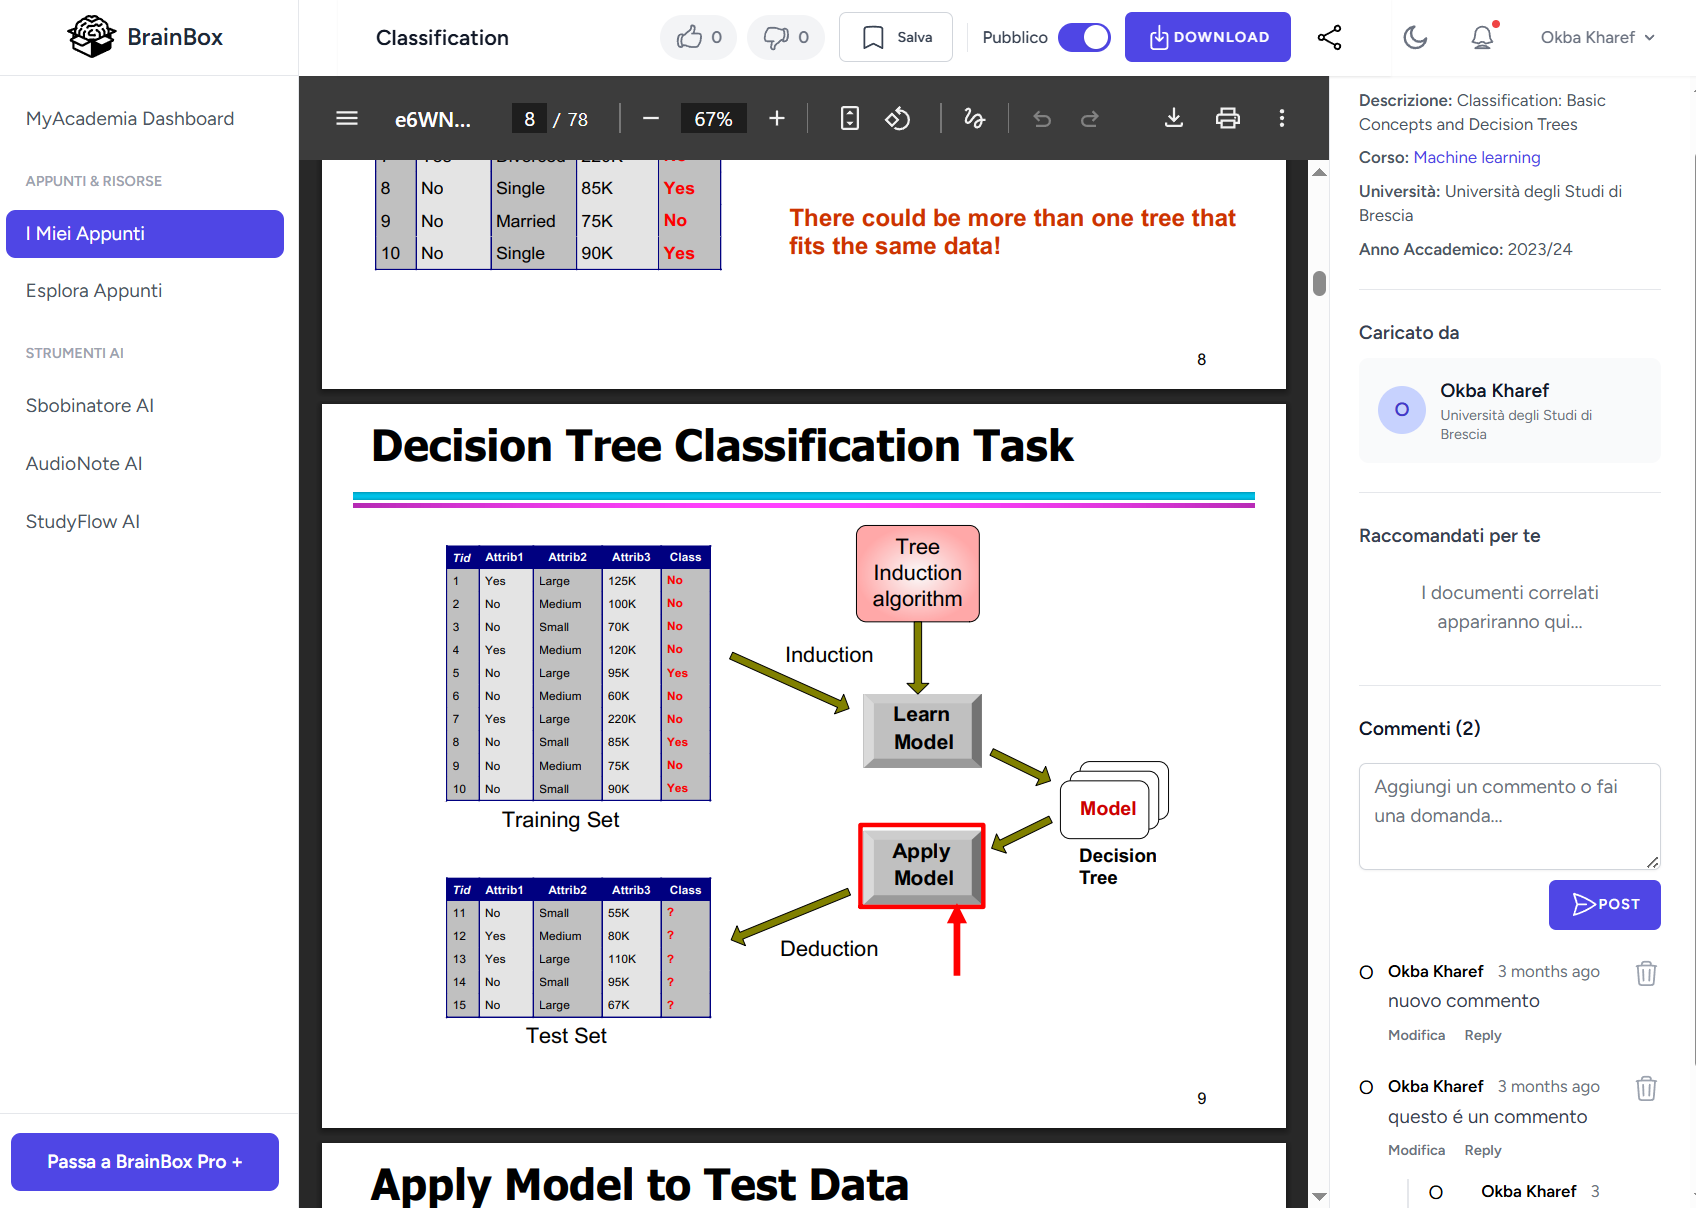
\includegraphics[width=0.8\textwidth]{figures/01-introduzione/immagine_14.png}
        \caption{Panoramica della Pagina di \textit{Dettaglio del Documento}, che illustra la sua struttura a tre sezioni: i \textit{metadati} dell'appunto, il \textit{form di input} per i commenti e l'area di consultazione delle interazioni.}
        \label{fig:1-14}
    \end{figure}

\subsubsection{Sezioni degli Strumenti AI}
\label{strumentiAI}
L'accesso alle funzionalità di intelligenza artificiale è suddiviso in due interfacce dedicate:

\begin{itemize}
    \item \textbf{Pagina Sbobinatore AI}: Presenta un form essenziale per l'upload di un file audio. Una volta avviato il processo, la pagina fornisce un \textit{feedback} sullo stato dell'elaborazione e, al termine, presenta la trascrizione testuale generata.
    
    \begin{figure}[H]
        \centering
        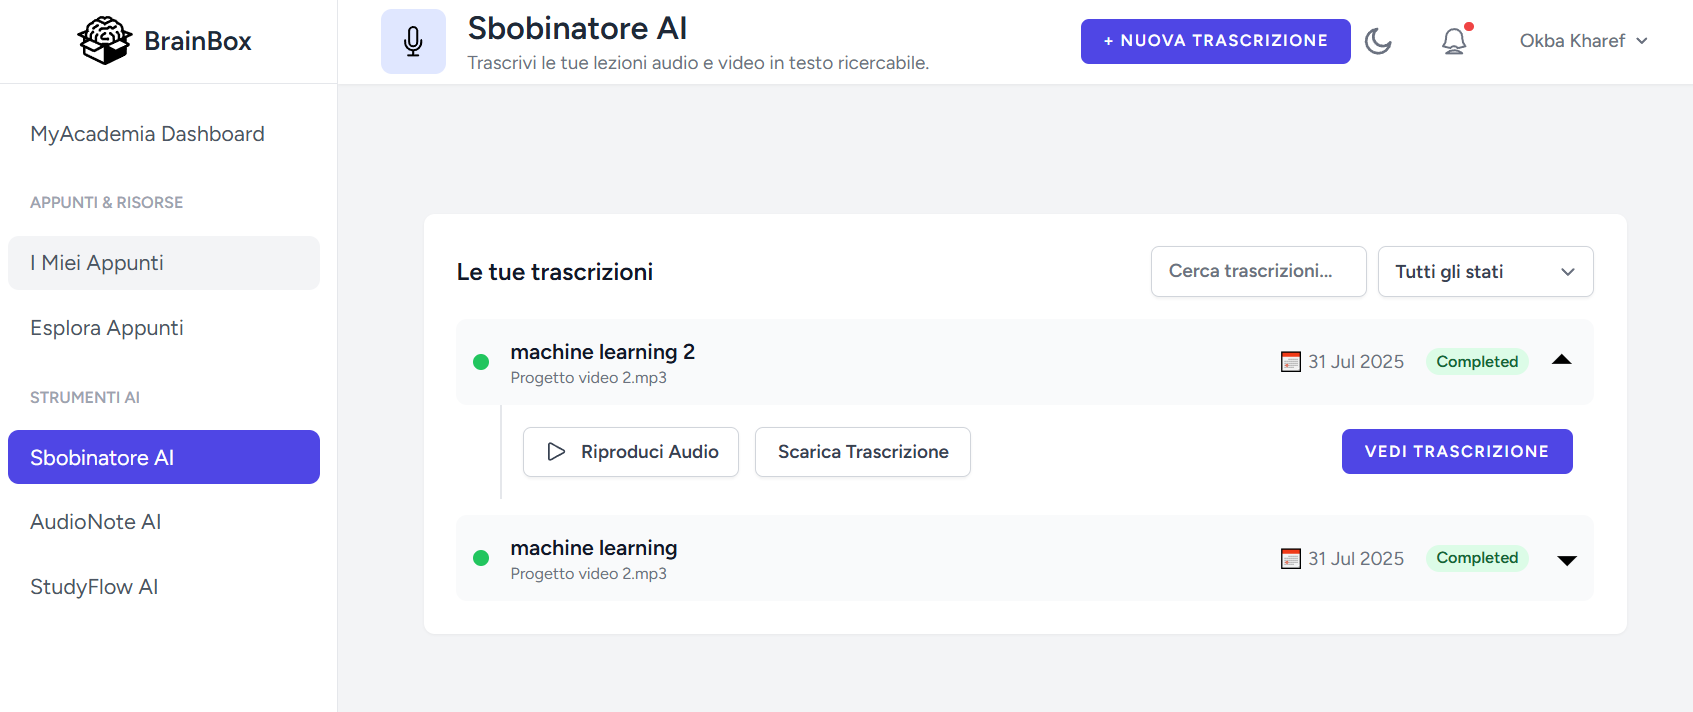
\includegraphics[width=0.8\textwidth]{figures/01-introduzione/immagine_15.png}
        \caption{Pagina principale dello \textit{Sbobinatore AI}, che mostra l'elenco delle trascrizioni precedenti dell'utente e il pulsante di azione per avviare una nuova trascrizione.}
        \label{fig:1-15}
    \end{figure}

    \begin{figure}[H]
        \centering
        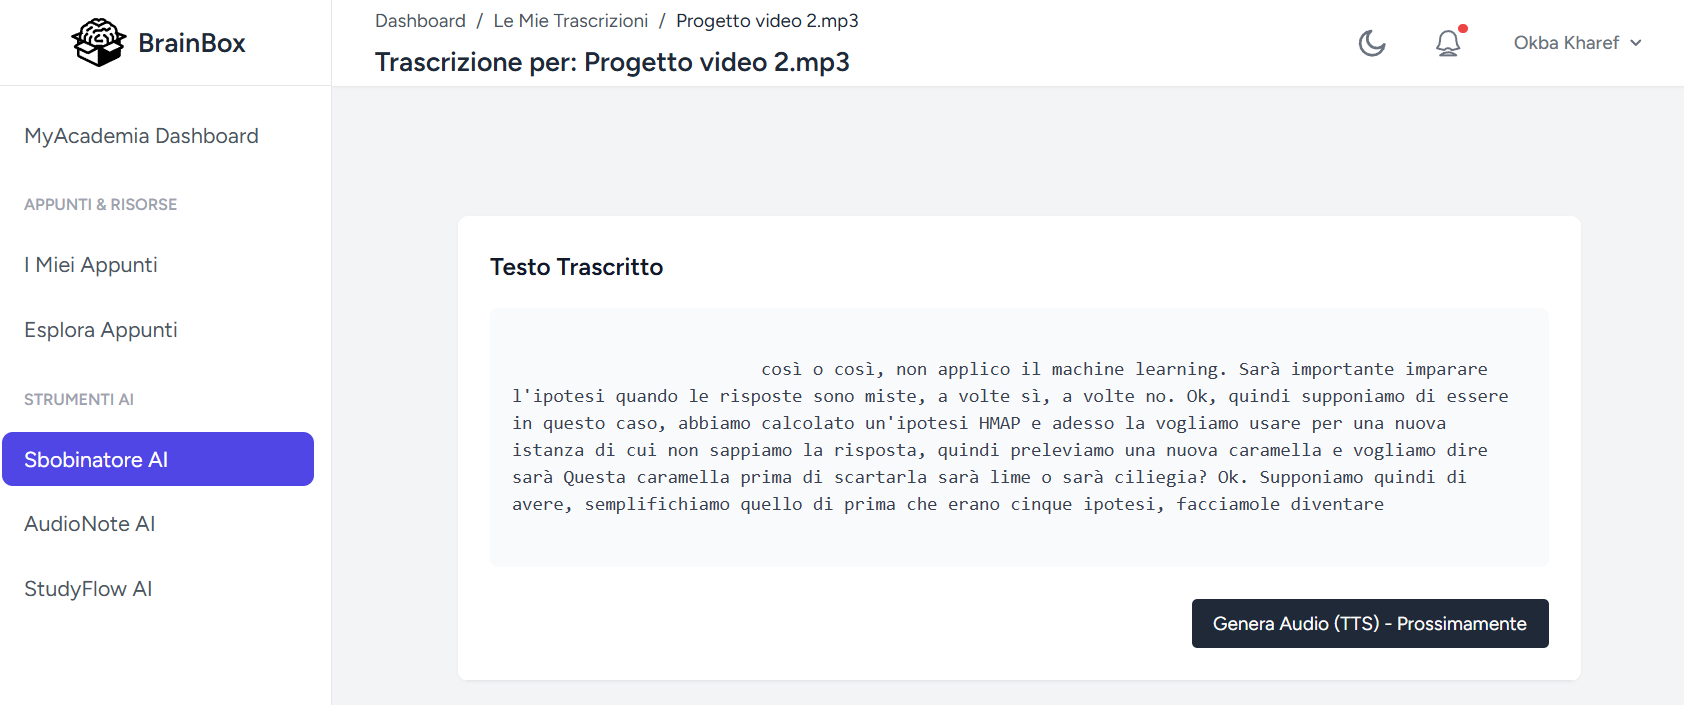
\includegraphics[width=0.8\textwidth]{figures/01-introduzione/immagine_16.png}
        \caption{Schermata finale del processo di trascrizione, in cui viene presentato all'utente il testo generato dal servizio AI a partire dal file audio.}
        \label{fig:1-16}
    \end{figure}
    
    \item \textbf{Pagina Generatore AudioNote}: Contiene un'area di testo (\textit{textarea}) in cui l'utente può inserire o incollare un contenuto testuale. Un pulsante di azione avvia il processo di sintesi vocale, rendendo disponibile per l'ascolto o il download il file audio risultante.
    
    \begin{figure}[H]
        \centering
        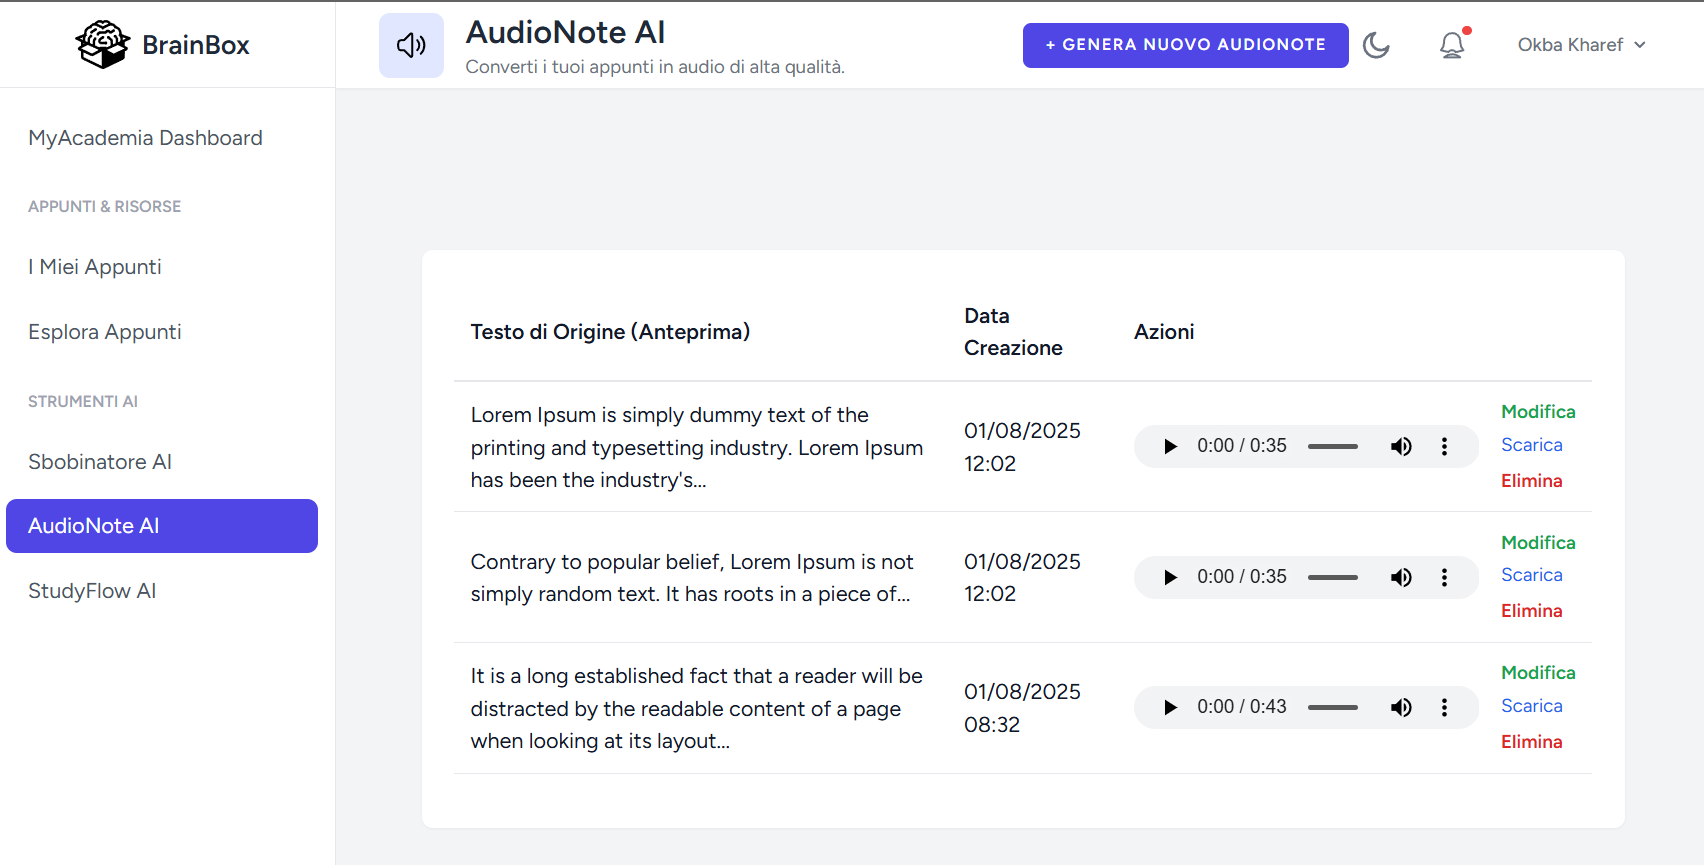
\includegraphics[width=0.8\textwidth]{figures/01-introduzione/immagine_17.png}
        \caption{Pagina principale dello \textit{AudioNote AI}, che mostra l'elenco degli audio precedenti dell'utente.}
        \label{fig:1-17}
    \end{figure}

    \begin{figure}[H]
        \centering
        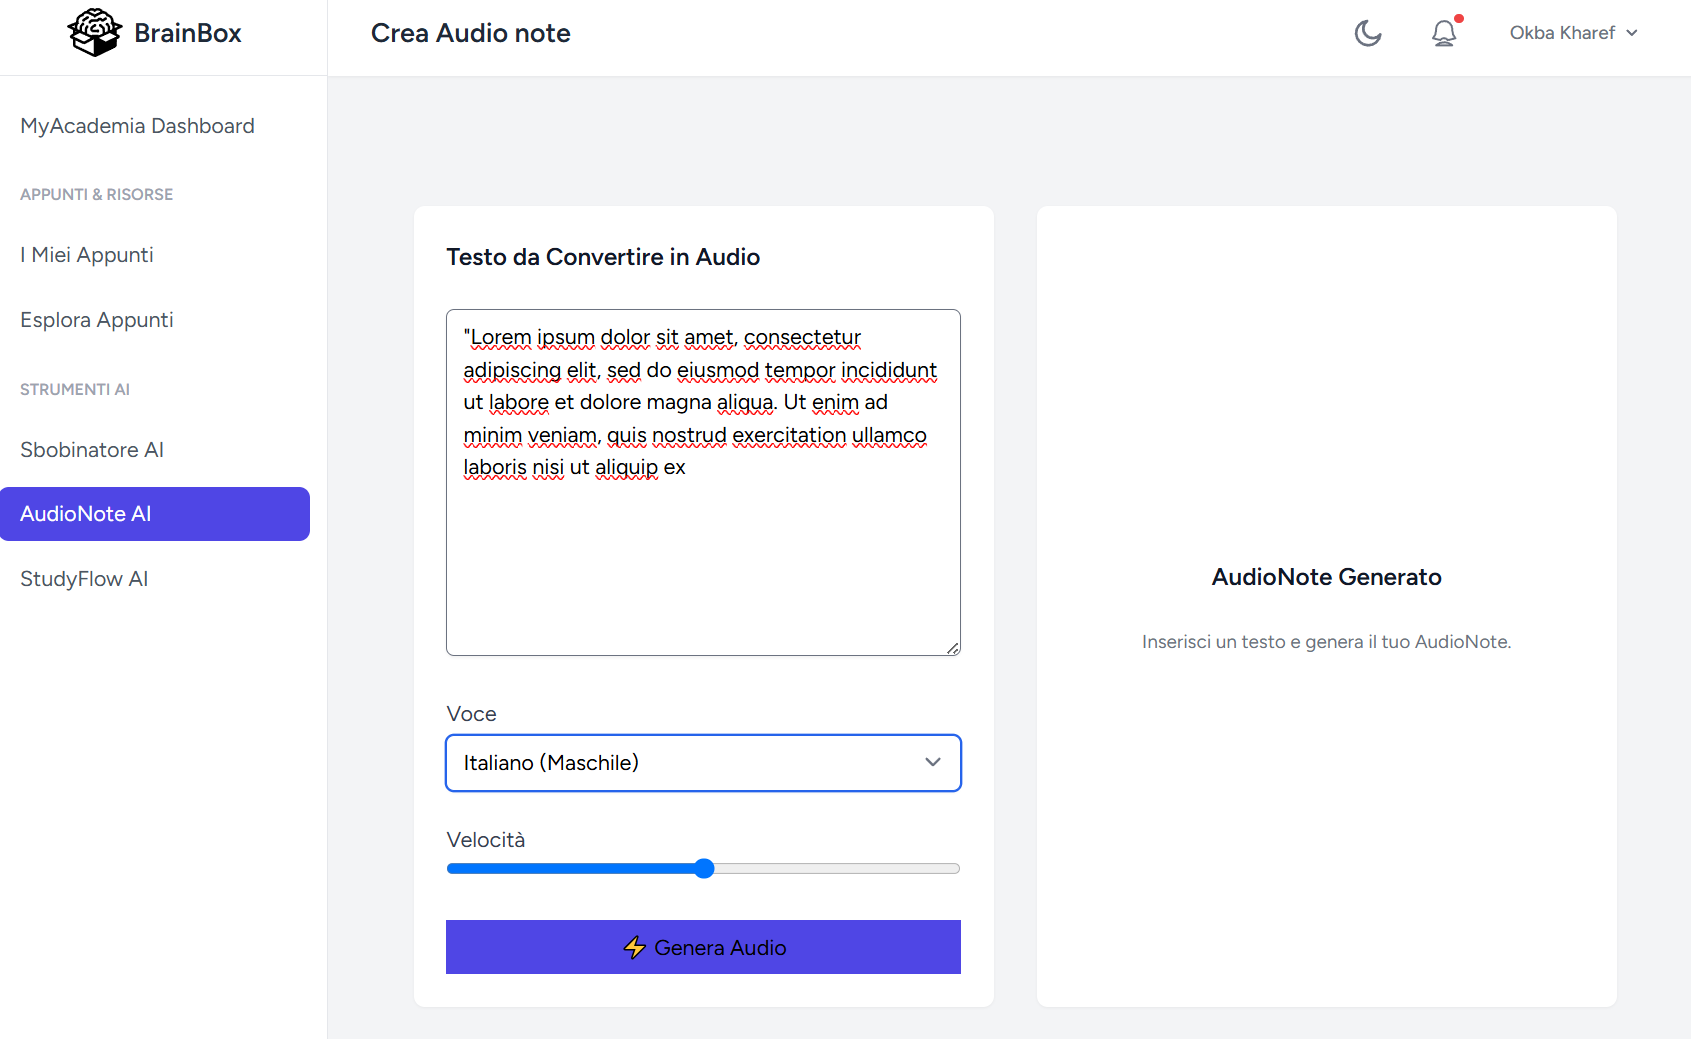
\includegraphics[width=0.8\textwidth]{figures/01-introduzione/immagine_18.png}
        \caption{Interfaccia del generatore AudioNote.}
        \label{fig:1-18}
    \end{figure}
\end{itemize}

\subsubsection{Sezione Profilo Utente}
\label{profilo_utente}
Questa sezione, accessibile tramite il menu a tendina associato al nome utente nella barra di navigazione, è dedicata alla gestione dell'account. L'interfaccia presenta i form standard per la modifica delle informazioni personali (nome, \textit{email}) e per l'aggiornamento sicuro della \textit{password}.

    \begin{figure}[H]
        \centering
        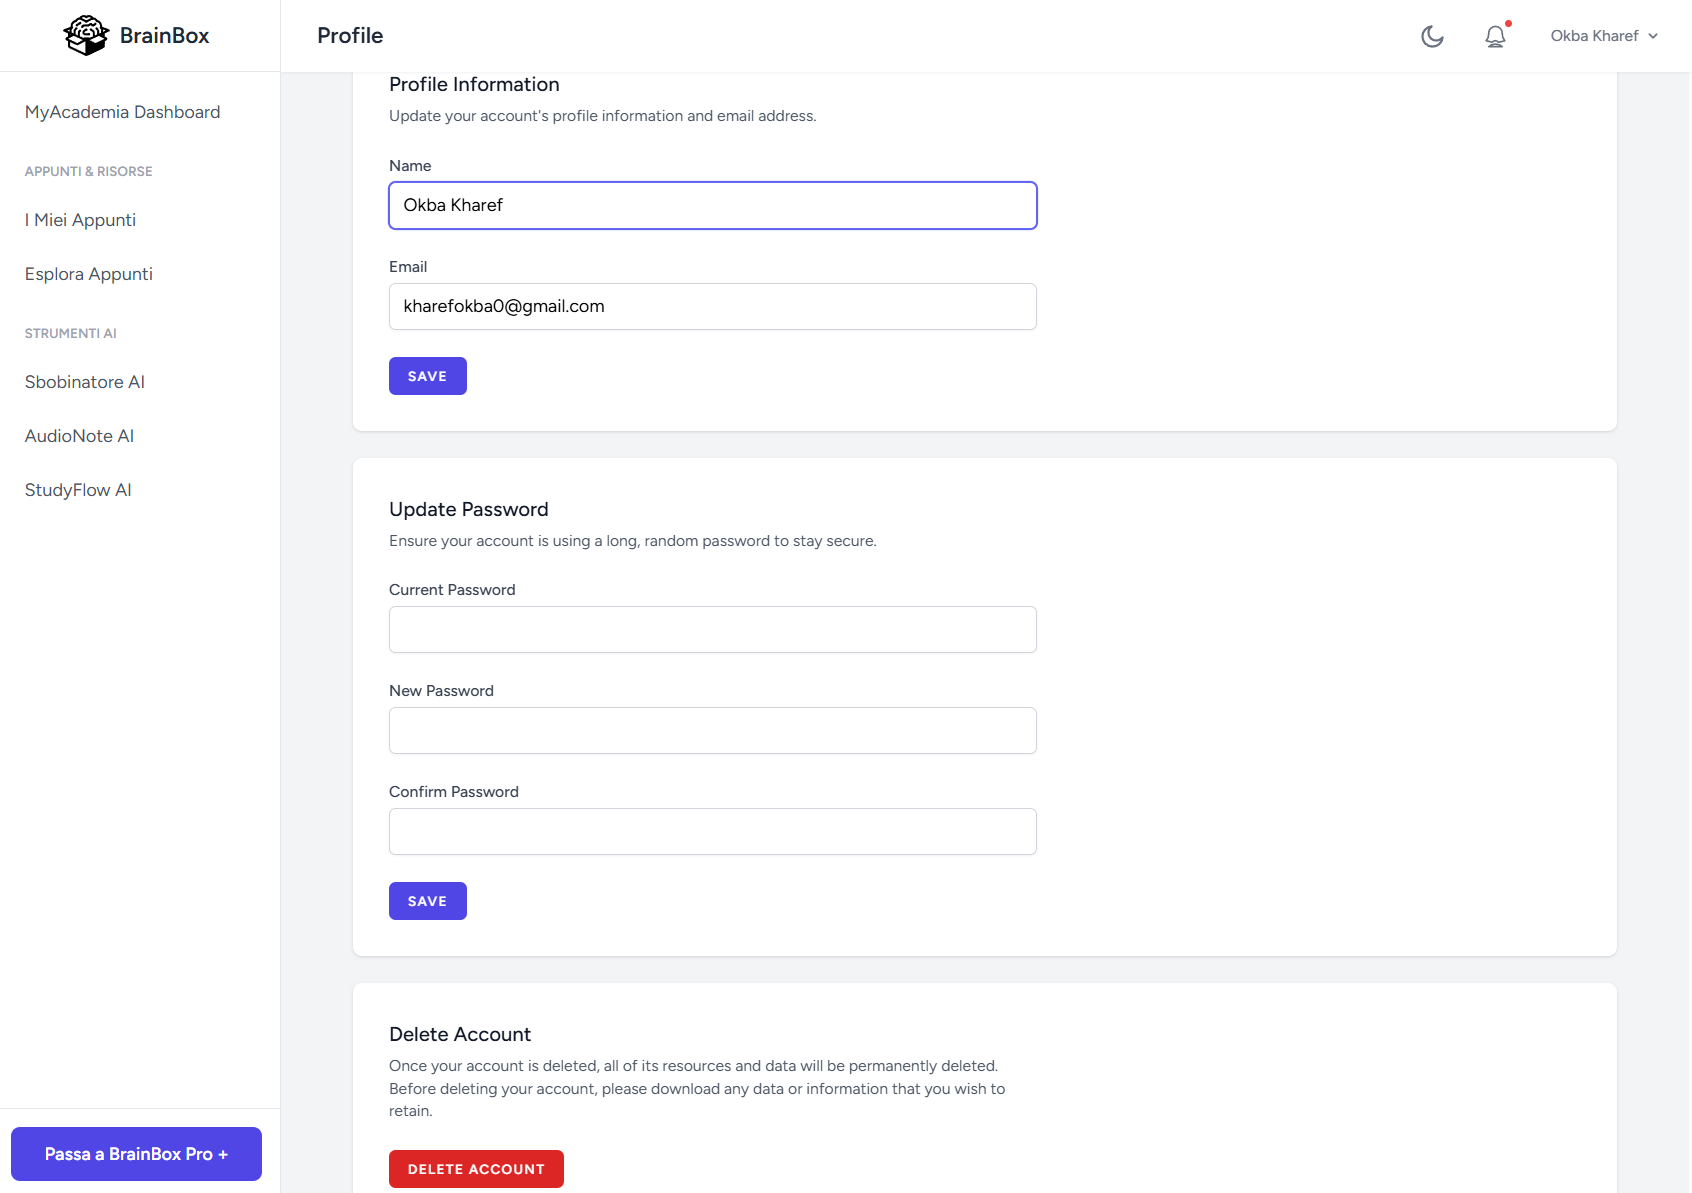
\includegraphics[width=0.8\textwidth]{figures/01-introduzione/immagine_19.png}
        \caption{Panoramica della pagina \textit{Profilo Utente}.}
        \label{fig:1-19}
    \end{figure}

\subsubsection{Sezione StudyFlow}
\label{study_flow}
Questa sezione è dedicata alla pianificazione strategica dello studio. Il suo scopo è fornire all'utente uno strumento per organizzare la preparazione degli esami in modo strutturato.

\begin{itemize}
    \item L'interfaccia principale presenta un elenco di tutti i \textit{Piani Esame} creati dall'utente. Ogni piano funziona come un contenitore per le attività relative a una specifica materia. Dalla pagina iniziale (Figura \ref{fig:1-20}), l'utente può creare un nuovo piano o accedere ai dettagli di uno esistente.
    
    \begin{figure}[H]
        \centering
        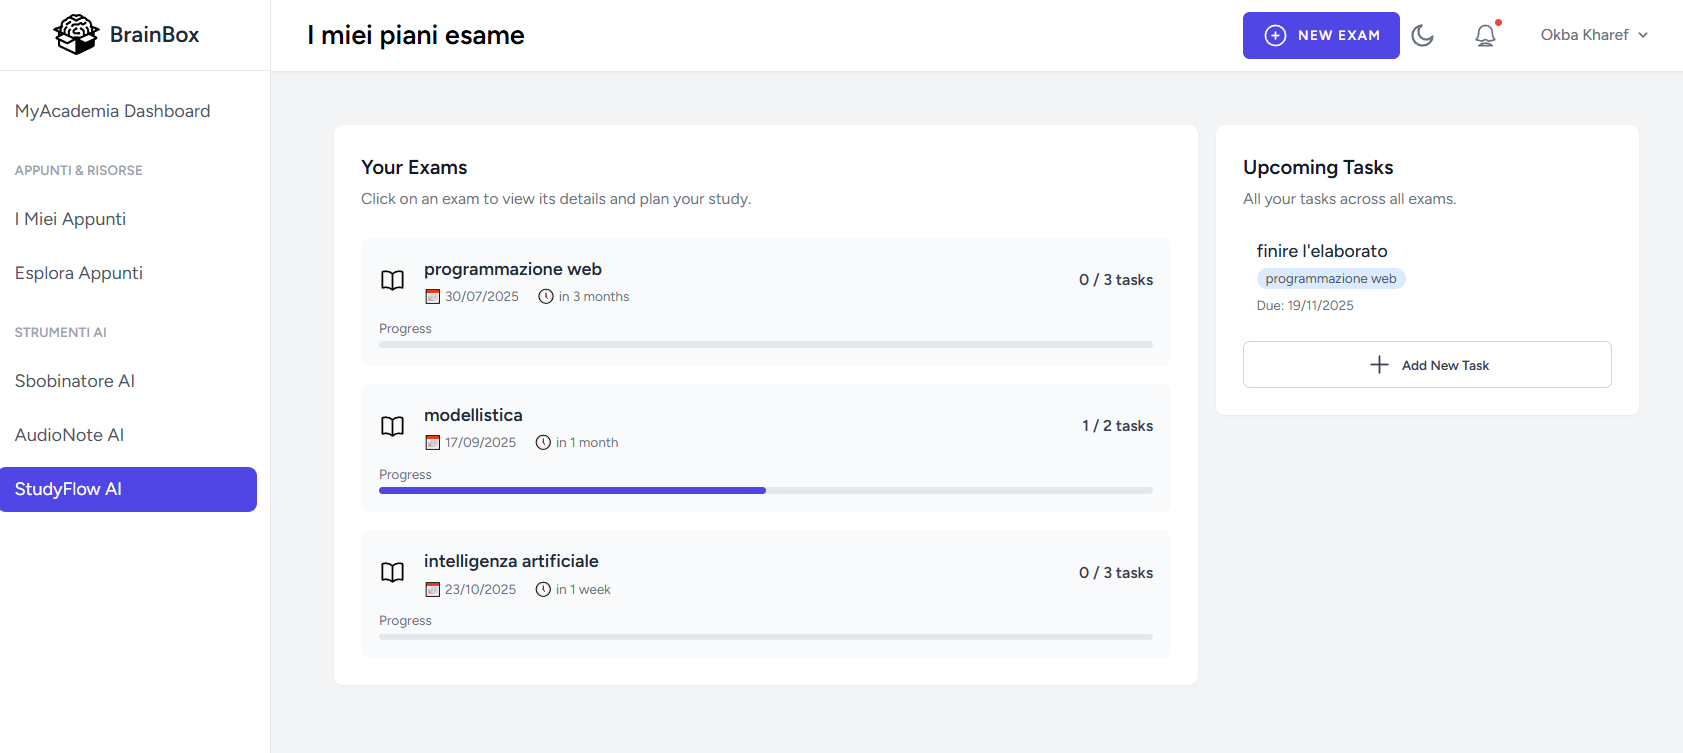
\includegraphics[width=0.8\textwidth]{figures/01-introduzione/immagine_20.png}
        \caption{Pagina principale della sezione \textit{StudyFlow AI}.}
        \label{fig:1-20}
    \end{figure}
    
    \item La pagina di dettaglio di un singolo \textit{Piano Esame} (Figura \ref{fig:1-21}) riassume le informazioni chiave (nome della materia, data dell'esame) e presenta l'elenco dei \textit{task} di studio associati: da qui l'utente può aggiungerne di nuovi, segnare quelli esistenti come completati, e collegare a ciascuno di essi le risorse di studio pertinenti, come gli appunti caricati in precedenza nella sezione (\ref{miei_appunti}) \textit{I Miei Appunti}.
    
    \begin{figure}[H]
        \centering
        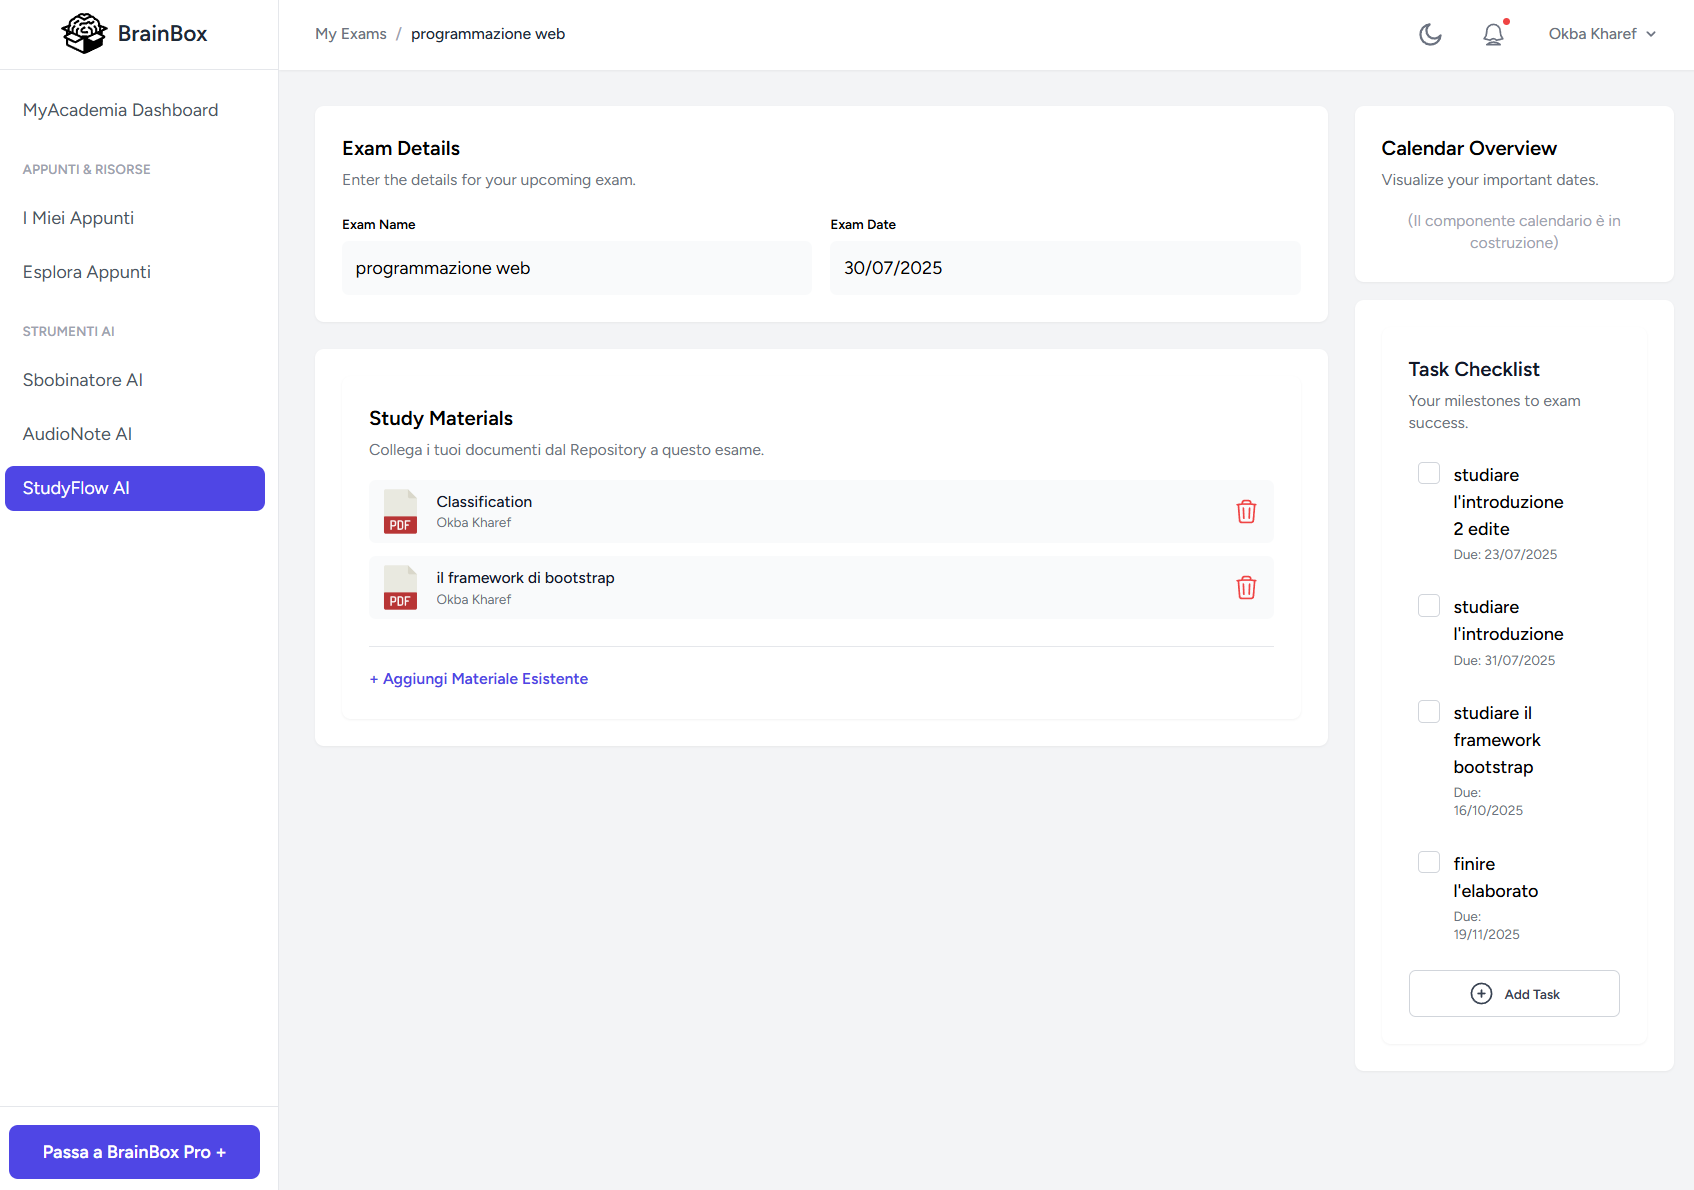
\includegraphics[width=0.8\textwidth]{figures/01-introduzione/immagine_21.png}
        \caption{Interfaccia di dettaglio di un \textit{Piano Esame}.}
        \label{fig:1-21}
    \end{figure}
\end{itemize}